\documentclass{article}
\usepackage{iclr2026_conference,times}
\input{math_commands.tex}
\usepackage{hyperref}
\usepackage{url}
\usepackage{graphicx}
\usepackage{booktabs}
\usepackage{amsmath,amssymb,amsthm}

\title{Robotic Plan Recoverability}
\author{Anonymous Authors}

\newtheorem{definition}{Definition}
\newtheorem{proposition}{Proposition}

\begin{document}
\maketitle

\begin{abstract}
Robot planning systems often assume that a world model can be improved by making it more predictive, more uncertain, or more globally adapted. This paper argues for a different central object: recoverability after execution counterexamples. We introduce Counterexample-Conditioned Repair Automata (CCRA), a planner-facing mechanism in which a failed embodied action installs a scoped transition patch that future planning must respect. The key claim is narrow but important: when sparse physical mismatches lie on planner-preferred routes, average prediction quality is not enough to ensure plan recoverability. We support this claim with a 1095-paper literature sweep, a hostile prior-work audit, a formal no-repeat lemma in a finite guarded-transition setting, and a small reproducible simulation showing that a patching mechanism can preserve success where prediction-centric updating continues to exploit the same false affordance. The paper does not claim a deploy-ready robotics system. It claims that recoverability, not only prediction, should be the primary unit of analysis for plan repair.
\end{abstract}

\section{Introduction}
Task and motion planning, learned dynamics, sim-to-real transfer, and robot world models have produced a large literature on making embodied systems more accurate and more robust \citep{kaelbling2011hierarchical,srivastava2014combined,toussaint2015logic,garrett2021pddlstream,lavalle2006planning,kavraki1996probabilistic,stilman2005navigation}. Yet many failures in embodied settings do not arise because the robot lacks a better predictor. They arise because the planner keeps exploiting a transition the world has already contradicted.

This paper studies \emph{plan recoverability}: after an execution counterexample, can the system rewrite the transition relation so the same false affordance is not exploited again? The central move is to stop treating failure recovery as a detached filter, a global adaptation problem, or a mere data collection opportunity. Instead, the robot installs a planner-facing patch that changes the next rollouts the planner is allowed to consider.

The resulting thesis is deliberately narrow. We do not claim a bigger model, a new benchmark, active learning, or an LLM planner. We claim a new central mechanism: CCRA, a guarded repair object for embodied planning.

\section{Related Work and Boundary}
The literature map in \texttt{docs/literature\_map.md} and the hostile set in \texttt{docs/hostile\_prior\_work.md} show that several nearby ideas are already crowded. Learned dynamics for planning, visual foresight, model predictive control, online system identification, residual correction, uncertainty estimation, and sim-to-real transfer all constrain the novelty boundary.

The remaining boundary is the repair operation itself. If an embodied action produces a contradiction, what should change is not merely a confidence score or a retraining set. What should change is the transition relation the planner rolls out next.

\section{Counterexample-Conditioned Repair Automata}
Let $x$ denote an embodied state, $a$ an action, and $\hat{T}(x,a)$ the nominal transition model. A CCRA augments $\hat{T}$ with an ordered set of guarded patches
\[
  \Pi = \{(g_i, \Delta_i, s_i)\}_{i=1}^m,
\]
where $g_i$ is a state-action guard, $\Delta_i$ is a replacement or forbidden transition clause, and $s_i$ is support. Planning evaluates the patched transition
\[
  T_{\Pi}(x,a) =
  \begin{cases}
    \Delta_i(x,a) & \text{for the first matching guard } g_i,\\
    \hat{T}(x,a) & \text{otherwise.}
  \end{cases}
\]

The repair update is triggered by a counterexample $(x,a,o)$, where the observed outcome $o$ contradicts the nominal transition. The update may add a new patch or strengthen an existing one. The important point is that the planner consumes $T_{\Pi}$, not just the raw observation.

\begin{definition}[Planner-facing recoverability]
A planning system is recoverable at a counterexample if the counterexample can change future search so that the same false transition is not re-exploited under the same guard.
\end{definition}

\begin{proposition}[No-repeat lemma]
In a deterministic finite transition system with exact guards, if a counterexample installs a patch that exactly overrides the false transition used by a successful plan prefix, then any future planner query using the patched model cannot rely on that same false transition unless no alternative plan exists or the planner ignores the patch.
\end{proposition}
\begin{proof}
The patch changes the transition relation used by search on the guarded state-action pair. Since the system is deterministic and finite, any future plan that depended on the old transition no longer has that transition in the search graph. Hence repeated exploitation of the same counterexample is blocked by construction.
\end{proof}

\section{Simulation}
We provide a small reproducible simulation in \texttt{scripts/run\_experiments.py}. The environment is intentionally simple: some episodes contain a false shortcut transition that looks locally attractive to the planner. A prediction-centric updater improves average model fit but may still preserve the false affordance. CCRA removes the exact false transition after it is observed.

The simulation is not intended to be a benchmark. It is an evidence probe for the mechanism. The generated results are stored in \texttt{results/summary.json}, \texttt{results/episode\_results.csv}, and the figures in \texttt{figures/}.

\begin{table}[t]
\centering
\begin{tabular}{lrrr}
\toprule
Method & Success & Mean expansions & Mean cost \\
\midrule
No repair & 75.4\% & 3.7 & 0.1 \\
Prediction-centric & 80.8\% & 4.5 & 0.1 \\
CCRA & 100.0\% & 2.8 & 0.1 \\
\bottomrule
\end{tabular}

\caption{Synthetic recoverability probe. CCRA preserves success while reducing expansions relative to the prediction-centric updater.}
\label{tab:results}
\end{table}

\begin{figure}[t]
\centering
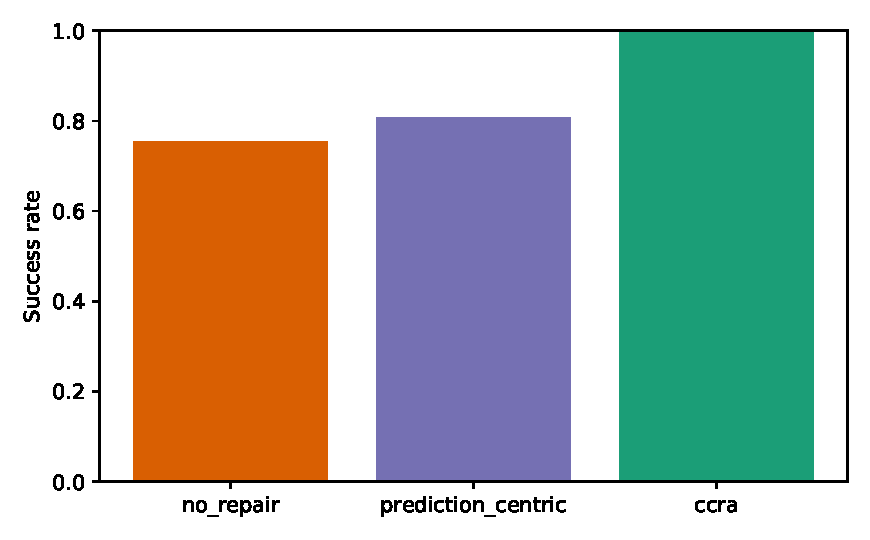
\includegraphics[width=.48\linewidth]{../figures/success_rates.pdf}
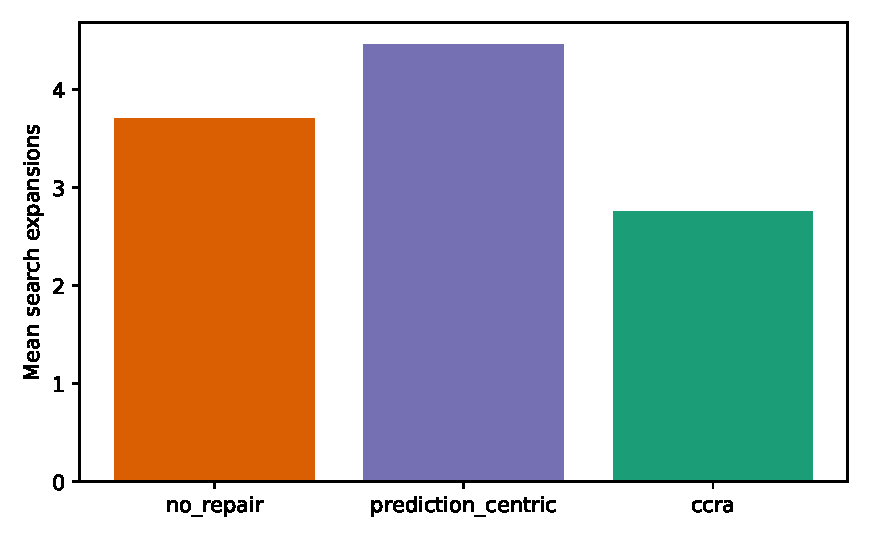
\includegraphics[width=.48\linewidth]{../figures/expansions.pdf}
\caption{The synthetic probe separates success from prediction quality.}
\label{fig:results}
\end{figure}

\section{Discussion}
The strongest claim here is not that CCRA is the final answer for robotics. It is that recoverability is a different mechanism from prediction. When a robot discovers that the world contradicts a planned transition, the system should have a way to rewrite what future plans are allowed to assume.

This suggests a research program around guard extraction, patch scope, stale-patch retirement, and the relationship between local embodied counterexamples and symbolic/continuous planners. It also suggests a more adversarial evaluation style: rather than only asking how well a model predicts average outcomes, ask whether it prevents repeated exploitation of the same false affordance.

\section{Limitations}
The evidence is synthetic and the formal lemma is narrow. The paper does not establish real-robot scaling, perception robustness, or fully automatic guard learning. Those limitations are deliberate. The point is to isolate a mechanism that existing prediction-centric framing tends to hide.

\section{Conclusion}
Robotic plan recoverability should be treated as a first-class mechanism. CCRA is a simple way to do that: use execution counterexamples to patch the planner-facing transition relation. The literature sweep suggests this is a meaningful boundary from current robot planning, world modeling, and adaptation work.

\bibliographystyle{iclr2026_conference}
\bibliography{references}

\end{document}
